\chapter{Zjawisko piezoelektryczne }
\label{sec:introduction}

Efekt piezoelektryczny został odkryty w 1880 r. przez Pierre’a i Jacques’a Curie. 
Podczas badań nad materiałami piroelektrycznymi odkryli, że naprężenia mechaniczne
generują ładunki na powierzchni badanych materiałów. Zjawisko piezoelektryczne 
występuje w materiałach krystalicznych. Pod wpływem zewnętrznych naprężeń mechanicznych 
dochodzi do odkształcenia struktury krystalicznej wzdłuż jednej z osi krystalograficznej, 
co skutukuje pojawieniem się ładunku na jej powierzchni. Dzieje się tak 
następuje defromacja powłok elektronowych oraz przemieszczenie jonów w krysztale.
Powoduje to gromadzenie się ładunków o przeciwnych znakach na przeciwległych
powierzchniach materiału piezoelektrycznego. Zjawisko to nazywa się efetem 
piezoelektrycznym prostym \cite{To_Do}
% [Zastosowanie piezoelektrycznych czujników PVDF do rejestracji 
% czasowego profilu ciśnienia fal uderzeniowych ANTONI SARZYŃSKI]. 
Jednocześnie 
umieszczenie materiału piezoelektrycznego w polu elektrycznym poprzez przyłożenie 
do jego powierzchni również prowadzi do przemieszczenia ładunków w jego strukturze, 
co skutkuje deformacją pojedynczych kryształów składających się na cały materiał a tym 
samym odkształcenie elementu. Jest to odwrotne zjawisko piezoelektryczne \cite{To_Do}
% [Zastosowanie 
% piezoelektrycznych czujników PVDF do rejestracji czasowego profilu ciśnienia fal 
% uderzeniowych ANTONI SARZYŃSKI]. 
Powstawanie efektu piezoelektrycznego przedstawiono na rysunku nr \ref{fig:piezo_effect}

\begin{figure}[htbp]
\centering
\fbox{rysunek}
% 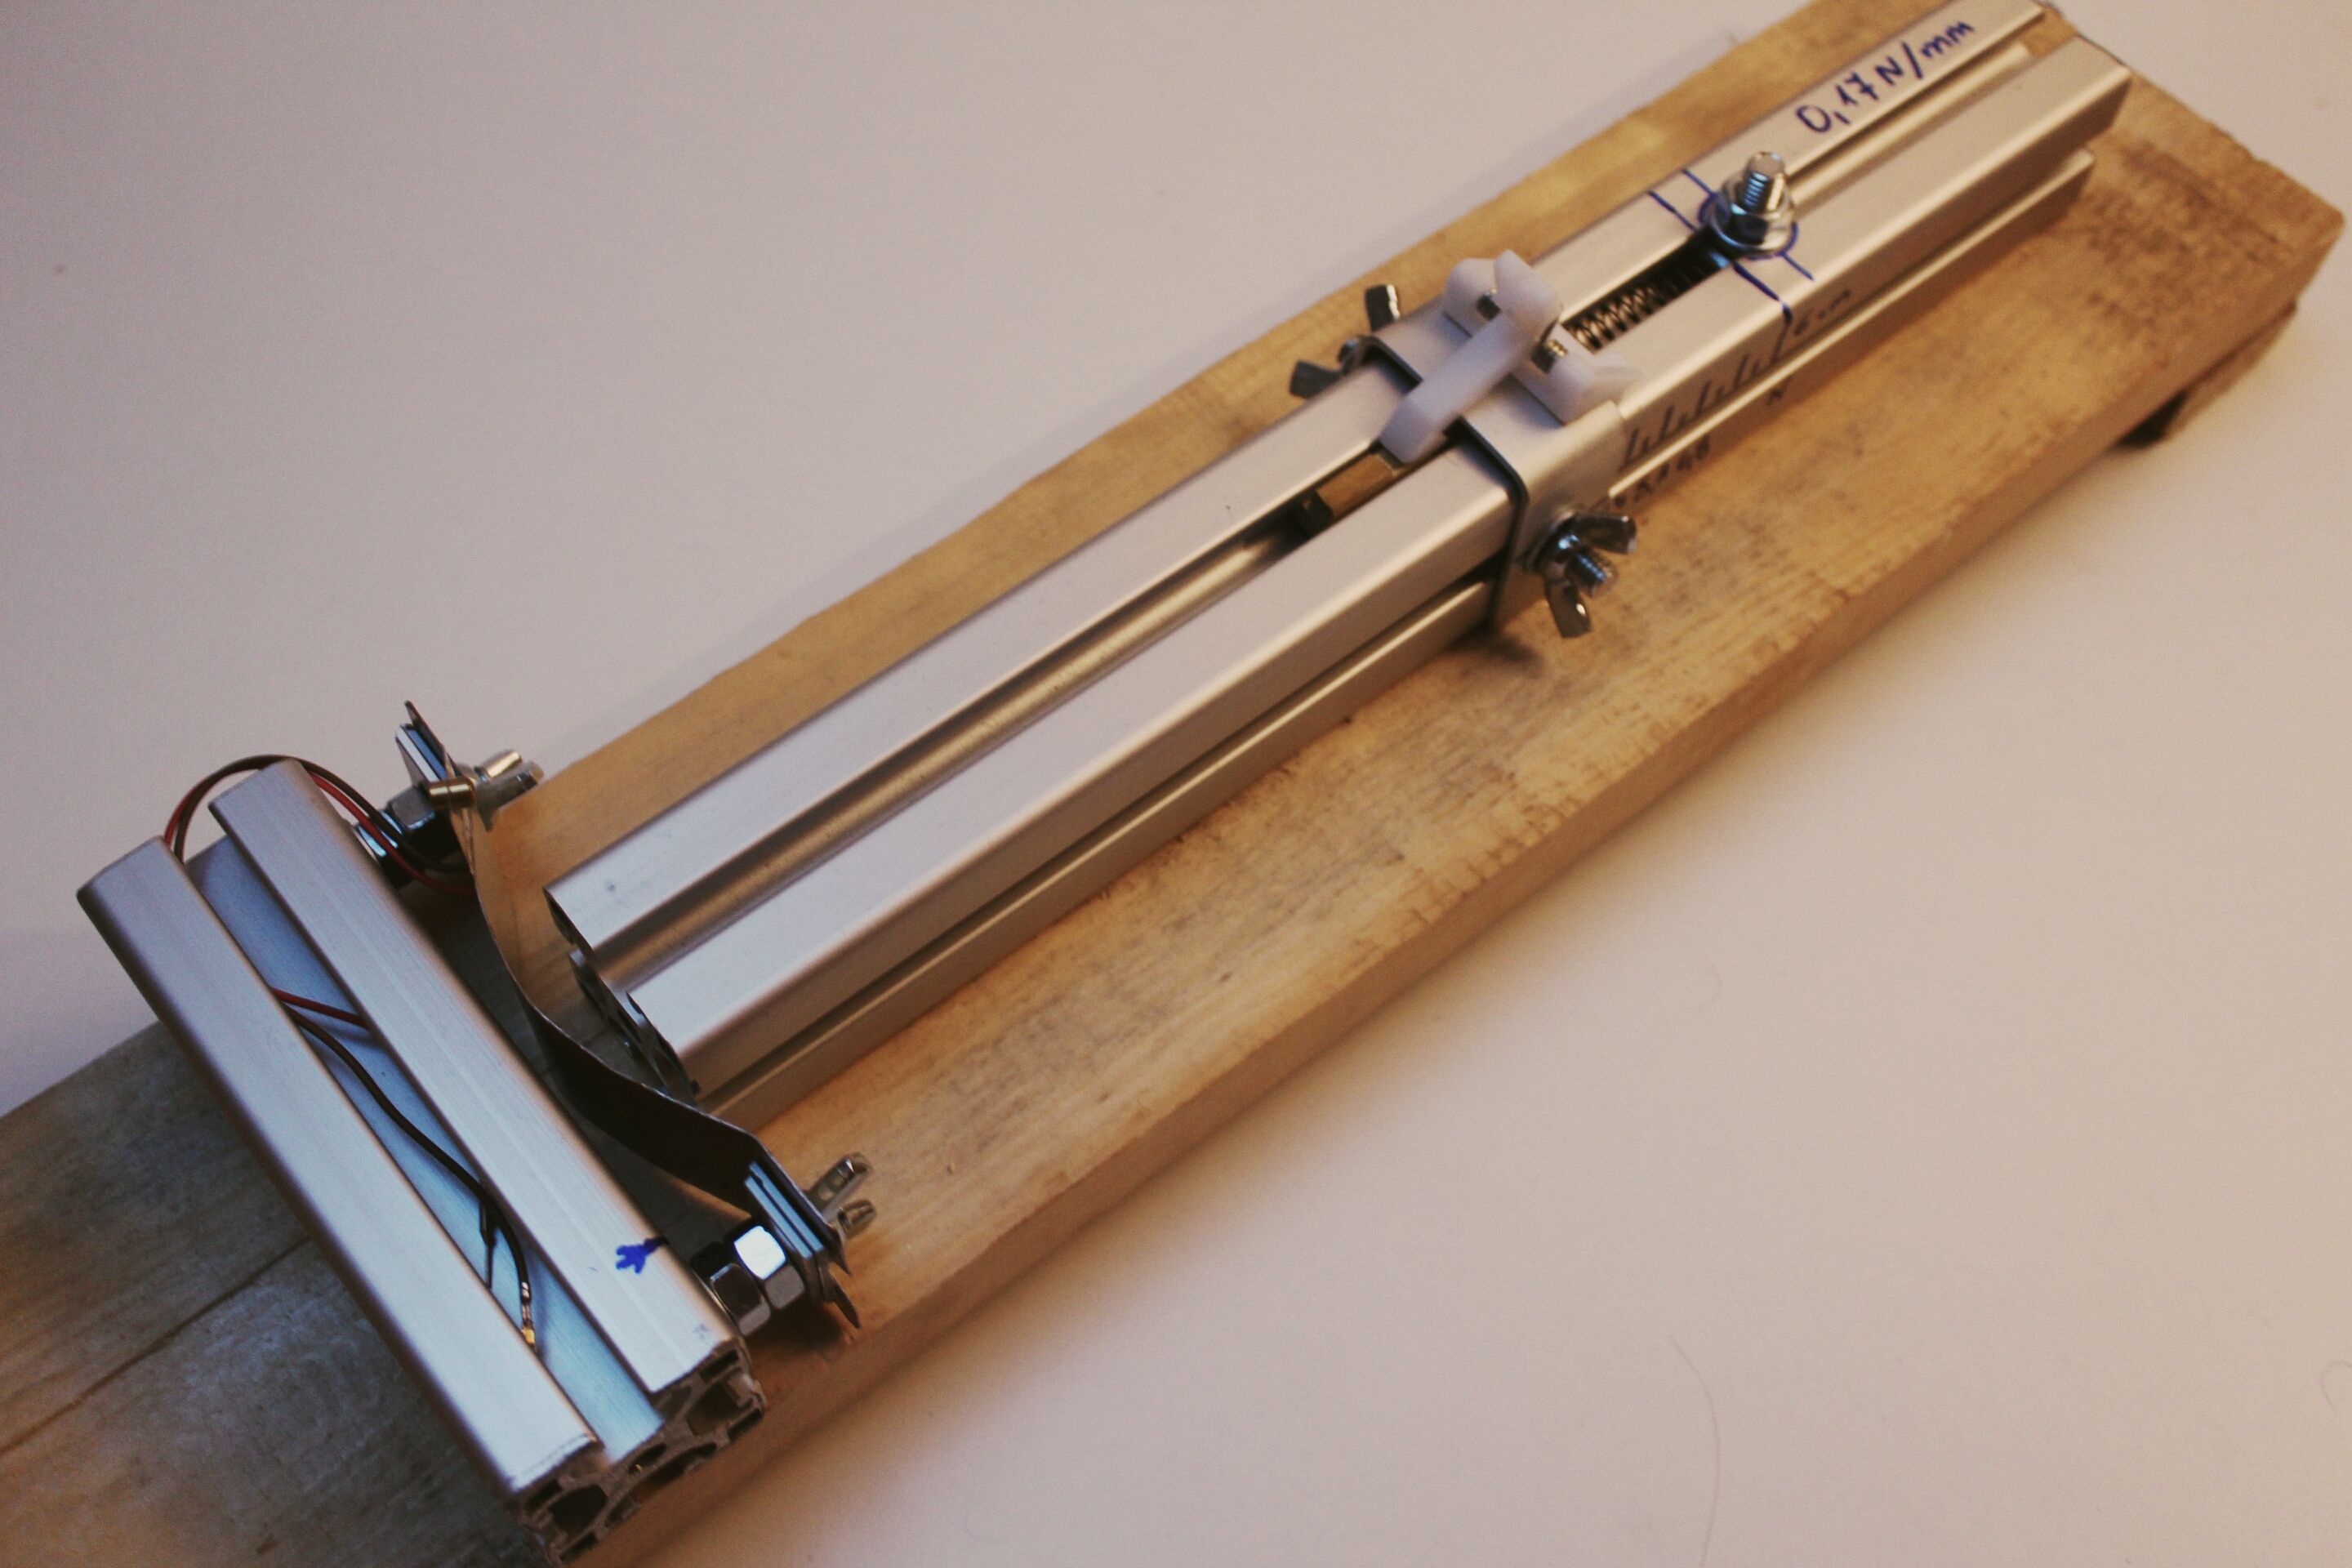
\includegraphics[width=\linewidth]{pictures/lab_stand.jpg}
\caption{Efekt piezoelektryczny występujący podczas ściskania kryształu. Źródło: \cite{To_Do}}
\label{fig:piezo_effect}
\end{figure}
% rys. Efekt piezoelektryczny występujący podczas ściskania kryształu [https://pl.wikipedia.org/wiki/Piezoelektryk]
Materiały, które wykazują efekt piezoelektryczny można podzielić na kryształy naturalne 
i syntetyczne, ceramikę piezoelektryczną oraz polimery piezoelektryczne. Naturalnymi 
materiałami piezoelektrycznymi są kryształy (kwarc, sól Rochelle, Turmaliny, Topaz, 
cukier trzcinowy, i niektóre substancje organiczne jak jedwab, drewno). Wśród ceramiki 
ferroelektrycznej wykazującej właściwości piezoelektryczne ceramiki polikrystaliczne 
takie jak tytanian baru (BaTiO3) i cyrkonian tytanian ołowiu są najbardziej popularnymi, 
w szczególności ze względu na niskie koszty produkcji i niemal dowolne możliwości 
kształtowania w stosunku do pojedynczego kryształu piezoelektrycznego. Ponadto 
charakteryzują się znakomitymi właściwościami piezoelektrycznymi i dielektrycznymi, 
które czynią je szczególnie przydatnymi jako materiał aktywny siłowników. Niestety wadą 
materiałów ceramicznych jest ich kruchość. Dlatego nie zawsze możliwe jest ich 
zastosowanie w systemach pomiaru udarów. Innymi materiałami wykazującymi bardzo dobre 
właściwości piezoelektryczne są polimery. Ich przewagą nad elementami ceramicznymi jest 
elastycznosć, co poszerza spektrum ich zastosowania. Do grupy piezoelektrycznych 
materiałów polimerowych zalicza się: polistyren, polipropylen, polimetakrylan metylu, 
semikrystaliczny poliamid, amorficzny octan winylu. Najsilniejszy efekt piezoelektryczny 
uzyskuje się dla polifluorku winylidenu (PVDF) oraz jego kopolimerów tj. trifluoroetylen,
tetrafluoroetylen \cite{To_Do}
% [www.ktech.com/research_development/applied_physics/The piezoelectric 
% properties of PVDF.pdf]
. Piezoelektryki wykonane z tego materiału są bardzo giętkie, co 
pozwala na dopasowanie ich kształtu do konkretnego urządzenia. Produkowane są w postaci 
cienkiej folii o grubości od kilku do klikuset mikrometrów. Czujniki piezoelektryczne 
produkowane z materiałów PVDF charakteryzują się bardzo dobrymi parametrami 
elektromechanicznymi. Mogą pracować w bardzo szerokim zakresie częstotliwości 
(od ułamków herców do setek gigaherców) oraz sił dynamicznych (ciścnienia w zakresie 
10-5 do 109 Pa). Również ogromną przewagą względem materiałów ceramicznych jest bardzo 
wysokie napięcie wyjściowe (dziesięciokrotnie wyższe przy tym samym wymuszeniu 
mechanicznym) \cite{To_Do}
% [J. S. Harrison, Z. Ounaies, Piezoelectric Polymers, NASA Report No. 
% 2001-43, http://www.teccenter.org/ electroactive_polymers/assets/pdfs/piezo polymers/icase_piezo.pdf]. 
Ze względu na swoje własności zarówno PVDF jak i jego kopolimery znalazły zastosowanie 
zwłaszcza w medycynie do wytwarzania sztucznych mięśni, skóry i organów ludzkich, 
urządzeń monitorujących m.in. przepływ krwi lub stan powierzchni skóry, sond do badań 
inwazyjnych, jak np. w transrektalnym USG, mikrofonów, inwazyjnych także w innych 
dziedzinach np. do wytwarzania podwodnych przetworników akustycznych, sejsmografów, 
pomp i zaworów, czujników natężenia ruchu drogowego, przełączników, akceleratorów, 
przetworników drgań, detektorów emisji akustycznych \cite{To_Do}
% [F. Bauer, PVDF Shock Sensors: 
% Applications to Polar Materials and High Explosives, IEEE Transactionson Ultrasonics, 
% Ferroelectrics, and Frequency Control, vol. 47, no. 6, 2000, 1448-1454].





\section{Nakreślenie celu pracy}
\label{sec:thesis_goal}
Podstawą przeprowadzonych badań jest ocena możliwości \textbf{konstrukcji przetwornika 
piezoelektrycznego} dla konkretnego przemysłowego zastosowania opisanego w rozdziale
\ref{sec:assumptions}. Analiza pozyskanych danych skupia się na optymalizowanym
w kolejnych krokach rozwiązaniu. Pobocznym celem jest przedstawienie perspektyw użycia
projektowanego rozwiązania konstrukcyjnego w szeroko rozumianym przemyśle. Stąd jednym
z zaplanowanych działań jest wyznaczenie charakterystyk mechaniczno-elektrycznych dla 
wybranych rozwiązań konstrukcyjnych. 

\section{Przegląd zagadnień teoretycznych}
\label{sec:theory}

TODO
Do napisania wprowadzenie. Zjawisko piezoelektryczne. 
Artykuł ma pokazać metodykę projektowania sensorów na konkretnym przykładzie.